


%\part{Escalado multidimensional.}
%\frame{\partpage}

\chapter{Escalado Multidimensional}

\section{Introducción}



\begin{frame}
\frametitle{Introducción}

\begin{itemize}
\item<2->{Las técnicas del escalado multidimensional son una generalización de las técnicas de componentes principales cuando se tiene una matriz $\vect{D}$ $n\times n$ de distancias o similaridades en lugar de una matriz de observaciones.}
\item<3->{El objetivo de nuestro análisis es representar dicha matriz mediante un conjunto de variables ortogonales $\vect{y}_1,\ldots,\vect{y}_p$ que llamaremos coordenadas principales donde suponemos que $p<n$ de manera que las distancias euclídeas al cuadrado entre las coordenadas de los elementos respecto a estas variables sean iguales o lo más próximas posible.}
\end{itemize}
\end{frame}

\begin{frame}
\frametitle{Introducción}
\begin{itemize}
\item<2->{Dicho de forma más explícita, dada la matriz de distancias o similaridades $\vect{D}$, queremos obtener una matriz $\vect{Y}=(y_{ij})_{i=1,\ldots,n,j=1,\ldots,p}$  $n\times p$ que puede interpretarse como la matriz de datos de $p$ variables en los $n$ individuos y donde la distancia euclídea al cuadrado entre los $n$ individuos venga dada aproximadamente por la matriz $\vect{D}=(d_{ij}^2)_{i,j=1,\ldots,n}$. }
\item<3->{O sea, para todo $i,j=1,\ldots,n$, $d_{ij}^2 = \sum\limits_{k=1}^p (y_{ik}-y_{jk})^2$.}
\item<4->{El escalado multidimensional comparte con el análisis de componentes principales el objetivo de describir e interpretar los datos.}
\item<5->{Dicho análisis nos permitirá encontrar la estructura de los datos estudiando la similaridad de las observaciones, estudiando grupos entre las mismas, viendo si hay observaciones atípicas, etc.}
\end{itemize}
\end{frame}
\section{Obtención de la matriz de datos}
\begin{frame}
\frametitle{Pasos a realizar para la obtención de la matriz $\vect{Y}$}
\begin{itemize}
\item<2->{En el primer paso obtenemos una matriz auxiliar $\vect{Q}=(q_{ij})_{i,j=1,\ldots,n}$ $n\times n$ llamada matriz de similitud a partir de la matriz $\vect{D}=(d_{ij}^2)_{i,j=1,\ldots,n}$ usando la expresión:
$$
q_{ij} = -\frac{1}{2}\left(d_{ij}^2 -d_{i\bullet}^2 -d_{\bullet j}^2 +d_{\bullet\bullet}^2\right),
$$
donde:
$$
d_{i\bullet}=\frac{1}{n}\sum_{j=1}^n d_{ij}^2,\ d_{\bullet j}=\frac{1}{n}\sum_{i=1}^n d_{ij}^2,\ d_{\bullet \bullet}=\frac{1}{n^2}\sum_{i=1}^n\sum_{j=1}^n d_{ij}^2.
$$
Matricialmente: $\vect{Q}=-\frac{1}{2}\vect{P}\vect{D}\vect{P}$, donde la matriz $\vect{P}$ es $\vect{P}=\vect{\rm{Id}}-\frac{1}{n}\vect{1}\vect{1}^\top$.}
\end{itemize}
\end{frame}

\begin{frame}
\frametitle{Pasos a realizar para la obtención de la matriz $\vect{Y}$}
\begin{itemize}
\item<2->{En el segundo paso obtendremos la matriz $\vect{Y}$ a partir de la matriz de similitud $\vect{Q}$. Para ello, suponiendo que dicha matriz es definida positiva, podemos descomponerla como:
$$
\vect{Q}=\vect{V}\cdot \vect{\Lambda}\cdot\vect{V}^{\top},
$$
donde $\vect{V}$ es $n\times p$ y contiene los vectores propios correspondientes a valores propios no nulos de la matriz~$\vect{Q}$ y $\vect{\Lambda}$ es diagonal $p\times p$ y contiene los valores propios no nulos de~$\vect{Q}$.}
\end{itemize}
\end{frame}

\begin{frame}
\frametitle{Pasos a realizar para la obtención de la matriz $\vect{Y}$}
\begin{itemize}
\item<2->{Usando que los valores propios de la matriz $\vect{Q}$ son positivos, podemos escribir:
$$
\vect{Q}=\left(\vect{V}\cdot \vect{\Lambda}^{1/2}\right)\left(\vect{\Lambda}^{1/2}\cdot\vect{V}^{\top}\right).
$$}
\item<3->{Sea $\vect{Y}=\vect{V}\cdot \vect{\Lambda}^{1/2}$. Dicha matriz es $n\times p$ y reproduce la métrica inicial~$\vect{D}$. Las columnas de dicha matriz son las variables $\vect{y}_1,\ldots,\vect{y}_p$ ortogonales que queríamos obtener.}
\end{itemize}
\end{frame}
\section{Propiedades de la matriz obtenida $\vect{Y}$}
\begin{frame}
\frametitle{Propiedades de la matriz obtenida $\vect{Y}$}
\begin{itemize}
\item<2->{La matriz obtenida por el método descrito anteriormente no es única.}
\item<3->{De hecho, si cogemos una matriz de datos $\vect{X}=(x_{ij})_{i=1,\ldots,n,j=1,\ldots,p}$ $n\times p$, calculamos una matriz de distancias entre sus elementos (filas) usando la expresión:
$$
d_{ij}^2=\sum_{s=1}^p (x_{is}-x_{js})^2,
$$
y aplicamos el método descrito anteriormente, lo más probable es que no obtengamos la matriz original $\vect{X}$. O sea, en general $\vect{Y}\not = \vect{X}$.}
\end{itemize}
\end{frame}
\begin{frame}
\frametitle{Propiedades de la matriz obtenida $\vect{Y}$}
\begin{itemize}
\item<2->{La razón de que no se obtenga la matriz original es que no existe una biyección entre una matriz de datos y una matriz de distancias calculada como se ha indicado anteriormente.}
\item<3->{Dada una matriz de datos $\vect{X}$, la matriz de distancias obtenida a partir de dicha matriz no varía si:
\begin{itemize}
\item<4->{modificamos las medias de las variables,}
\item<5->{rotamos los puntos. O sea, multiplicamos la matriz $\vect{X}$ por una matriz ortogonal.}
\end{itemize}}
\end{itemize}
\end{frame}
\begin{frame}
\frametitle{Ejemplo}
\begin{itemize}
\item<2->{Consideremos la siguiente matriz de distancias entre $10$ proteínas:
{\tiny 
\begin{center}
$$\left(\begin{array}{rrrrrrrrrr}
0.00, & 0.09, & 0.17, & 0.19, & 0.15, & 0.08, & 0.05, & 0.20, & 0.07, & 0.18 \\
0.09, & 0.00, & 0.17, & 0.17, & 0.06, & 0.09, & 0.06, & 0.14, & 0.04, & 0.11 \\
0.17, & 0.17, & 0.00, & 0.05, & 0.20, & 0.13, & 0.17, & 0.11, & 0.16, & 0.16 \\
0.19, & 0.17, & 0.05, & 0.00, & 0.20, & 0.13, & 0.18, & 0.13, & 0.16, & 0.17 \\
0.15, & 0.06, & 0.20, & 0.20, & 0.00, & 0.15, & 0.12, & 0.14, & 0.10, & 0.08 \\
0.08, & 0.09, & 0.13, & 0.13, & 0.15, & 0.00, & 0.06, & 0.17, & 0.06, & 0.17 \\
0.05, & 0.06, & 0.17, & 0.18, & 0.12, & 0.06, & 0.00, & 0.18, & 0.03, & 0.15 \\
0.20, & 0.14, & 0.11, & 0.13, & 0.14, & 0.17, & 0.18, & 0.00, & 0.16, & 0.07 \\
0.07, & 0.04, & 0.16, & 0.16, & 0.10, & 0.06, & 0.03, & 0.16, & 0.00, & 0.14 \\
0.18, & 0.11, & 0.16, & 0.17, & 0.08, & 0.17, & 0.15, & 0.07, & 0.14, & 0.00 \\
\end{array}\right)
$$
\end{center}
}
}
\end{itemize}
\end{frame}
\begin{frame}
\frametitle{Ejemplo}
\begin{itemize}
\item<2->{Calculamos la matriz de similitud $\vect{Q}$. Para ello, primero tenemos que hallar la matriz $\vect{P}$:
{\tiny
\begin{center}
$$
\left(\begin{array}{r@{}r@{}r@{}r@{}r@{}r@{}r@{}r@{}r@{}r}
0.90, & -0.10, & -0.10, & -0.10, & -0.10, & -0.10, & -0.10, & -0.10, & -0.10, & -0.10 \\
 -0.10, & 0.90, & -0.10, & -0.10, & -0.10, & -0.10, & -0.10, & -0.10, & -0.10, & -0.10 \\
 -0.10, & -0.10, & 0.90, & -0.10, & $-$0.10, & -0.10, & -0.10, & -0.10, & -0.10, & -0.10 \\
 -0.10, & -0.10, & -0.10, & 0.90, & -0.10, & -0.10, & -0.10, & -0.10, & -0.10, & -0.10 \\
 -0.10, & -0.10, & -0.10, & -0.10, & 0.90, & -0.10, & -0.10, & -0.10, & -0.10, & -0.10 \\
 -0.10, & -0.10, & -0.10, & -0.10, & -0.10, & 0.90, & -0.10, & -0.10, & -0.10, & -0.10 \\
  -0.10, & -0.10, & -0.10, & -0.10, & -0.10, & -0.10, & 0.90, & -0.10, & -0.10, & -0.10 \\
 -0.10, & -0.10, & -0.10, & -0.10, & -0.10, & -0.10, & -0.10, & 0.90, & -0.10, & -0.10 \\
 -0.10, & -0.10, & -0.10, & -0.10, & -0.10, & -0.10, & -0.10, & -0.10, & 0.90, & -0.10 \\
 -0.10, & -0.10, & -0.10, & -0.10, & -0.10, & -0.10, & -0.10, & -0.10, & -0.10, & 0.90 \\
\end{array}\right)
$$\end{center}}
$\vect{Q}$ será entonces: $\vect{Q}=-\frac{1}{2}\vect{P}\vect{D}\vect{P}$.
}
\end{itemize}
\end{frame}
\begin{frame}
\frametitle{Ejemplo}
\begin{itemize}
\item<2->{La matriz $\vect{Q}$ será en este caso:
{\tiny 
\begin{center}
$$\left(
\begin{array}{r@{}r@{}r@{}r@{}r@{}r@{}r@{}r@{}r@{}r}
0.06,  &  0.00,  &  -0.02,  &  -0.02,  &  -0.01,  &  0.01,  &  0.03,  &  -0.03,  &  0.01,  &  -0.03 \\
0.00,  &  0.04,  &  -0.03,  &  -0.03,  &  0.02,  &  -0.00,  &  0.01,  &  -0.02,  &  0.01,  &  -0.00 \\
-0.02,  &  -0.03,  &  0.07,  &  0.05,  &  -0.03,  &  -0.00,  &  -0.03,  &  0.02,  &  -0.03,  &  -0.01 \\
-0.02,  &  -0.03,  &  0.05,  &  0.08,  &  -0.03,  &  -0.00,  &  -0.03,  &  0.01,  &  -0.02,  &  -0.01 \\
-0.01,  &  0.02,  &  -0.03,  &  -0.03,  &  0.06,  &  -0.02,  &  -0.01,  &  -0.00,  &  -0.00,  &  0.02 \\
0.01,  &  -0.00,  &  -0.00,  &  -0.00,  &  -0.02,  &  0.05,  &  0.01,  &  -0.03,  &  0.01,  &  -0.03 \\
0.03,  &  0.01,  &  -0.03,  &  -0.03,  &  -0.01,  &  0.01,  &  0.04,  &  -0.03,  &  0.02,  &  -0.02 \\
-0.03,  &  -0.02,  &  0.02,  &  0.01,  &  -0.00,  &  -0.03,  &  -0.03,  &  0.07,  &  -0.03,  &  0.03 \\
0.01,  &  0.02,  &  -0.03,  &  -0.02,  &  -0.00,  &  0.01,  &  0.02,  &  -0.03,  &  0.03,  &  -0.02 \\
-0.03,  &  -0.00,  &  -0.01,  &  -0.01,  &  0.02,  &  -0.03,  &  -0.02,  &  0.03,  &  -0.02,  &  0.07 \\
\end{array}\right)$$
\end{center}}}
\item<3->{Los valores propios de la matriz $\vect{Q}$ son aproximadamente:
{\tiny\begin{center}
$$
\begin{array}{rrrrrrrrrr}
0.22,  &  0.16,  &  0.05,  &  0.04,  &  0.03,  &  0.03,  &  0.02,  &  0.02,  &  0.01,  &  0.00 \\
\end{array}
$$
\end{center}}}
\end{itemize}
\end{frame}

\begin{frame}
\frametitle{Ejemplo}
\begin{itemize}
\item<2->{Sólo vamos a tener en cuenta los 9 primeros valores propios ya que el último es nulo. Los vectores propios correspondientes a estos 9 valores propios son:
{\tiny\begin{center}
$$
\left(\begin{array}{r@{}r@{}r@{}r@{}r@{}r@{}r@{}r@{}r}
-0.33,  &  -0.22,  &  0.41,  &  0.64,  &  0.00,  &  -0.15,  &  -0.33,  &  0.07,  &  0.16 \\
-0.23,  &  0.17,  &  -0.29,  &  -0.11,  &  -0.42,  &  -0.10,  &  -0.12,  &  0.65,  &  -0.30 \\
0.44,  &  -0.34,  &  -0.03,  &  0.26,  &  -0.16,  &  -0.15,  &  0.67,  &  0.14,  &  0.03 \\
0.44,  &  -0.36,  &  -0.40,  &  0.04,  &  0.06,  &  0.33,  &  -0.53,  &  -0.11,  &  -0.07 \\
-0.10,  &  0.48,  &  -0.51,  &  0.28,  &  0.15,  &  -0.35,  &  0.07,  &  -0.42,  &  0.02 \\
-0.17,  &  -0.31,  &  0.02,  &  -0.47,  &  0.60,  &  -0.41,  &  0.00,  &  0.13,  &  -0.01 \\
-0.35,  &  -0.12,  &  0.17,  &  -0.08,  &  -0.05,  &  0.39,  &  0.24,  &  -0.39,  &  -0.60 \\
0.41,  &  0.28,  &  0.49,  &  -0.31,  &  -0.34,  &  -0.31,  &  -0.23,  &  -0.25,  &  -0.05 \\
-0.29,  &  -0.06,  &  -0.09,  &  -0.32,  &  -0.30,  &  0.28,  &  0.11,  &  -0.13,  &  0.71 \\
0.20,  &  0.50,  &  0.23,  &  0.07,  &  0.45,  &  0.47,  &  0.10,  &  0.33,  &  0.10 \\
\end{array}\right)
$$
\end{center}}
}
\item<3->{La matriz anterior será la matriz $\vect{V}$ del algoritmo.}
\end{itemize}
\end{frame}
\begin{frame}
\frametitle{Ejemplo}
\begin{itemize}
\item<2->{Puede comprobarse que, en este caso: $\vect{Q}=\vect{V}\vect{\Lambda}\vect{V}^\top$, donde {\small $$\vect{\Lambda}={\rm diag}(0.22,  0.16,  0.05,  0.04,  0.03,  0.03,  0.02,  0.02,  0.01).$$}}
\item<3->{Las coordenadas principales serán:
{\tiny 
$$
\vect{Y}=\vect{V}\vect{\Lambda}^{1/2}=\left(\begin{array}{r@{}r@{}r@{}r@{}r@{}r@{}r@{}r@{}r}
-0.15,  &  -0.09,  &  0.10,  &  0.13,  &  0.00,  &  -0.02,  &  -0.05,  &  0.01,  &  0.02 \\
-0.11,  &  0.07,  &  -0.07,  &  -0.02,  &  -0.07,  &  -0.02,  &  -0.02,  &  0.08,  &  -0.03 \\
0.20,  &  -0.14,  &  -0.01,  &  0.05,  &  -0.03,  &  -0.02,  &  0.10,  &  0.02,  &  0.00 \\
0.20,  &  -0.14,  &  -0.09,  &  0.01,  &  0.01,  &  0.05,  &  -0.08,  &  -0.01,  &  -0.01 \\
-0.05,  &  0.19,  &  -0.12,  &  0.06,  &  0.03,  &  -0.06,  &  0.01,  &  -0.05,  &  0.00 \\
-0.08,  &  -0.13,  &  0.01,  &  -0.09,  &  0.11,  &  -0.07,  &  0.00,  &  0.02,  &  -0.00 \\
-0.16,  &  -0.05,  &  0.04,  &  -0.02,  &  -0.01,  &  0.06,  &  0.04,  &  -0.05,  &  -0.06 \\
0.19,  &  0.11,  &  0.11,  &  -0.06,  &  -0.06,  &  -0.05,  &  -0.03,  &  -0.03,  &  -0.01 \\
-0.14,  &  -0.02,  &  -0.02,  &  -0.06,  &  -0.05,  &  0.04,  &  0.02,  &  -0.02,  &  0.08 \\
0.09,  &  0.20,  &  0.05,  &  0.01,  &  0.08,  &  0.08,  &  0.01,  &  0.04,  &  0.01 \\
\end{array}\right)
$$}}
\item<4->{Podemos comprobar que si hallamos la matriz de distancias al cuadrado de la matriz $\vect{Y}$ obtenemos la matriz inicial $\vect{D}$.}
\end{itemize}
\end{frame}

\section{Matrices compatibles con métricas euclídeas.}
\begin{frame}
\frametitle{Matrices compatibles con métricas euclídeas.}
\begin{itemize}
\item<2->{Para poder usar el algoritmo indicado anteriormente, necesitamos que la matriz $\vect{Q}$ sea semidefinida positiva o que no tenga ningún valor propio no negativo. Dicha condición no se cumple siempre.}
\item<3->{Diremos que una matriz de distancias $\vect{D}$ es compatible con una métrica euclídea si la matriz de similitud $\vect{Q}=-\frac{1}{2}\vect{P}\vect{D}\vect{P}$ obtenida a partir de ella es semidefinida positiva.}
\item<4->{Se puede demostrar que la condición anterior es necesaria y suficiente. O sea, si $\vect{D}$ se ha construido a partir de una métrica euclídea, $\vect{Q}$ es semidefinida positiva y si $\vect{Q}$ es semidefinida positiva, es posible encontrar una métrica euclídea que reproduzca $\vect{D}$.}
\end{itemize}
\end{frame}
\section{Caso de matrices no compatibles con métricas euclídeas}
\begin{frame}
\frametitle{Cálculo de las coordenadas principales en general.}
\begin{itemize}
\item<2->{En el caso en que la matriz de distancias $\vect{D}$ no sea compatible con métricas euclídeas, es posible en algunos casos hallar una aproximación de las coordenadas principales.}
\item<3->{Para hallar dicha aproximación, hay que realizar los pasos siguientes:}
\begin{itemize}
\item<4->{Hallar la matriz $\vect{Q}=-\frac{1}{2}\vect{P}\vect{D}\vect{P}$ de similitud.}
\item<5->{Obtener los valores propios de $\vect{Q}$. Aunque pueden aparecer valores propios negativos, es posible que existan $r$ valores propios positivos que en módulo sobresalgan sobre los anteriores. Si éste es el caso, tomamos estos $r$ valores propios.}
\item<6->{Sea $\vect{V}_r$ la matriz de los vectores propios correspondientes a los $r$ valores propios anteriores.}
\item<7->{Definimos la aproximación de las coordenadas principales como: $\vect{Y}_r \approx \vect{V}_r\vect{\Lambda}_r^{1/2}$, donde $\vect{\Lambda}_r$ es una matriz diagonal con los $r$ valores propios en la diagonal.}
\end{itemize}
\end{itemize}
\end{frame}

\begin{frame}
\frametitle{Ejemplo anterior}
\begin{itemize}
\item<2->{Aunque en el ejemplo anterior, la matriz de distancias $\vect{D}$ es compatible con métricas euclídeas, hallemos una aproximación de las coordenadas principales.}
\item<3->{En el cálculo de los valores propios de la matriz $\vect{Q}$ vimos que había dos que sobresalían sobre los demás. Éstos eran $0.22$ y $0.16$.}
\item<4->{La matriz $\vect{V}_r$ de vectores propios correspondiente a dichos valores propios es:
{\small $$\vect{V}_r =
\left(\begin{array}{rr}
-0.33 & -0.22 \\
-0.23 & 0.17 \\
0.44 & -0.34 \\
0.44 & -0.36 \\
-0.10 & 0.48 \\
-0.17 & -0.31 \\
-0.35 & -0.12 \\
0.41 & 0.28 \\
-0.29 & -0.06 \\
0.20 & 0.50 \\
\end{array}\right)
$$}
}
\end{itemize}
\end{frame}

\begin{frame}
\frametitle{Ejemplo anterior}
\begin{itemize}
\item<2->{La aproximación de las coordenadas principales será:
$$
\vect{Y}_r \approx \vect{V}_r\vect{\Lambda}_r^{1/2} =\left(\begin{array}{rr}
-0.33 & -0.22 \\
-0.23 & 0.17 \\
0.44 & -0.34 \\
0.44 & -0.36 \\
-0.10 & 0.48 \\
-0.17 & -0.31 \\
-0.35 & -0.12 \\
0.41 & 0.28 \\
-0.29 & -0.06 \\
0.20 & 0.50 \\
\end{array}\right) \left(\begin{array}{rr}
0.22 & 0.00 \\ 0.00 & 0.16
\end{array}\right)^{1/2}
$$}
\end{itemize}
\end{frame}

\begin{frame}
\frametitle{Ejemplo anterior}
\begin{itemize}
\item<2->{{\tiny $$
\vect{Y}_r \approx 
\left(
\begin{array}{rr}
-0.15 & $-$0.09 \\
$-$0.11 & 0.07 \\
0.20 & $-$0.14 \\
0.20 & $-$0.14 \\
$-$0.05 & 0.19 \\
$-$0.08 & $-$0.13 \\
$-$0.16 & $-$0.05 \\
0.19 & 0.11 \\
$-$0.14 & $-$0.02 \\
 0.09 & 0.20 \\
\end{array}\right)
$$}}
\item<3->{Definimos en general grado de bondad de la aproximación al valor:
$$
m=100\cdot \frac{\sum_{i=1}^r \lambda_i}{\sum_{i=1}^p |\lambda_i|}\%,
$$donde los $\lambda_i$ representan los valores propios de la matriz de similitud~$\vect{Q}$}
\end{itemize}
\end{frame}

\begin{frame}
\frametitle{Ejemplo anterior}
\begin{itemize}
\item<2->{El grado de bondad valdrá en nuestro caso:
\begin{eqnarray*}
m &= & 100\cdot \frac{0.22+0.16}{(0.22+0.16+0.05+0.04+\cdots +0.00)}\% \\
& = & 65.25\%
\end{eqnarray*}}
\item<3->{Podemos concluir que las dos variables tenidas en cuenta explican el $65.25\%$ de la variabilidad entre las proteínas.}
\end{itemize}
\end{frame}
\begin{frame}
\frametitle{Ejemplo anterior}
\begin{itemize}
\item{En el gráfico siguiente podemos ver la representación de la coordenadas principales halladas anteriormente:
\begin{center}
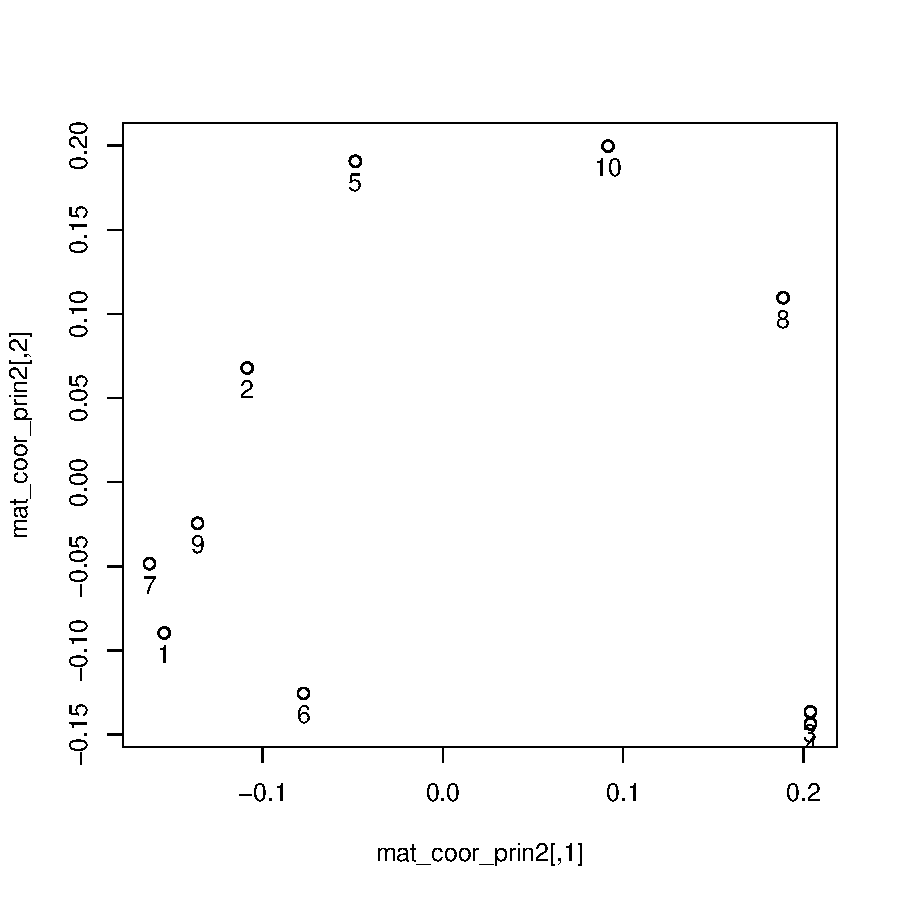
\includegraphics[scale=0.45]{EscalMulti.pdf}
\end{center}
}
\end{itemize}
\end{frame}
\section{Relación entre las coordenadas principales y las componentes principales}
\begin{frame}
\frametitle{Relación entre las coordenadas principales y las componentes principales}
\begin{itemize}
\item<2->{Sea $\vect{X}=({x}_{ij})_{i=1,\ldots,n,j=1,\ldots,p}$ una matriz de datos de $n$ datos y $p$ variables. Sea $\tilde{\vect{X}}$ la matriz centrada construida a partir de la matriz $\vect{X}$.}
\item<3->{Sea $\vect{D}=(d_{ij}^2)_{i,j=1,\ldots,n}$ la matriz de distancias euclídeas al cuadrado construidaa a partir de la matriz ${\vect{X}}$:
$$
d_{ij}^2 = \sum_{k=1}^p ({x}_{ik} -{x}_{jk})^2, \ \forall i,j=1\ldots,n.
$$ }
\item<4->{Entonces las coordenadas principales obtenidas de la matriz $\vect{D}$ son equivalentes a las componentes principales de la matriz $\vect{X}$ usando la matriz de covarianzas.}
\end{itemize}
\end{frame}

\begin{frame}
\frametitle{Relación entre las coordenadas principales y las componentes principales}
\begin{itemize}
\item<2->{Recordemos que las componentes principales se calculaban como: $\vect{CP}=\tilde{\vect{X}}\vect{u}$, donde $\vect{u}$ es la matriz de los vectores propios de la matriz de covarianzas (donde cada vector tiene módulo unidad) $\tilde{\vect{X}}^\top\tilde{\vect{X}}$.}
\item<3->{Sea $\vect{V}$ la matriz de vectores propios de la matriz $\tilde{\vect{X}}\tilde{\vect{X}}^\top$ correspondientes a valores propios no nulos (donde cada vector tiene módulo unidad). Sean $\lambda_1,\ldots,\lambda_p$ los valores propios no nulos. Entonces las coordenadas principales $\vect{Y}$ pueden calcularse como $\vect{Y}=\vect{V}\rm{diag}(\sqrt{\lambda_1},\ldots,\sqrt{\lambda_p})$. }
\end{itemize}
\end{frame}
\begin{frame}
\frametitle{Relación entre las coordenadas principales y las componentes principales}
\begin{itemize}
\item<2->{Puede demostrarse que si $\vect{u}$ es un vector propio de valor propio $\lambda$ de la matriz $\tilde{\vect{X}}^\top\tilde{\vect{X}}$, entonces $\tilde{\vect{X}}\vect{u}$ es un vector propio de la matriz $\tilde{\vect{X}}\tilde{\vect{X}}^\top$ con el mismo valor propio.}
\item<3->{Concluimos que tanto las componentes principales como las coordenadas principales son vectores propios de la matriz $\tilde{\vect{X}}\tilde{\vect{X}}^\top$. Por tanto, aparte de un factor de escala, las componentes principales y las coordenadas principales son iguales.}
\item<4->{Tanto en la técnica de componentes principales como en la técnica de coordenadas principales, tratamos de reducir la dimensionalidad de los datos.}
\item<5->{Como hemos visto, si la matriz de similaridades $\vect{Q}$ proviene de una métrica euclídea, ambos métodos son equivalentes. Sin embargo, la técnica de coordenadas principales puede aplicarse a un conjunto más general de problemas.}
\end{itemize}
\end{frame}
